\documentclass{standalone}
\usepackage{tikz}
\begin{document}
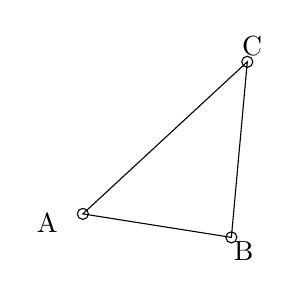
\begin{tikzpicture}[x=1pt,y=1pt]
\draw (137.93,-203.33) -- (191.59,-211.82) -- (197.35,-148.37) -- cycle;
\draw (137.94,-203.33) circle (2.00);
\draw (191.59,-211.82) circle (2.00);
\draw (197.35,-148.37) circle (2.00);
\node at (125.07,-206.58) {A};
\node at (199.09,-142.79) {C};
\node at (196.00,-216.87) {B};
\end{tikzpicture}
\end{document}
